% This example is meant to be compiled with lualatex or xelatex
% The theme itself also supports pdflatex
\PassOptionsToPackage{unicode}{hyperref}
\documentclass[aspectratio=1610, 12pt]{beamer}

% Warning, if another latex run is needed
% \usepackage[aux]{rerunfilecheck}

% just list chapters and sections in the toc, not subsections or smaller
\setcounter{tocdepth}{1}

%------------------------------------------------------------------------------
%------------------------------ Fonts, Unicode, Language ----------------------
%------------------------------------------------------------------------------
\usepackage{fontspec}
\defaultfontfeatures{Ligatures=TeX}  % -- becomes en-dash etc.

% german language
\usepackage{polyglossia}
\setdefaultlanguage{german}

% for english abstract and english titles in the toc
\setotherlanguages{english}

% intelligent quotation marks, language and nesting sensitive
\usepackage[autostyle]{csquotes}

% microtypographical features, makes the text look nicer on the small scale
\usepackage{microtype}

%------------------------------------------------------------------------------
%------------------------ Math Packages and settings --------------------------
%------------------------------------------------------------------------------

\usepackage{amsmath}
\usepackage{amssymb}
\usepackage{mathtools}
\usepackage{bbold}

% Enable Unicode-Math and follow the ISO-Standards for typesetting math
\usepackage[
  math-style=ISO,
  bold-style=ISO,
  sans-style=italic,
  nabla=upright,
  partial=upright,
]{unicode-math}
\setmathfont{Latin Modern Math}

% nice, small fracs for the text with \sfrac{}{}
\usepackage{xfrac}


%------------------------------------------------------------------------------
%---------------------------- Numbers and Units -------------------------------
%------------------------------------------------------------------------------

\usepackage[
  locale=DE,
  separate-uncertainty=true,
  per-mode=symbol-or-fraction,
]{siunitx}
\sisetup{math-micro=\text{µ},text-micro=µ}
% \sisetup{tophrase={{ to }}}
%------------------------------------------------------------------------------
%-------------------------------- tables  -------------------------------------
%------------------------------------------------------------------------------

\usepackage{booktabs}       % \toprule, \midrule, \bottomrule, etc

%------------------------------------------------------------------------------
%-------------------------------- graphics -------------------------------------
%------------------------------------------------------------------------------

\usepackage{graphicx}
%\usepackage{rotating}
\usepackage{grffile}
\usepackage{tikz}
\usepackage{circuitikz}
\usepackage{tikz-feynman}
\usepackage{subcaption}

% allow figures to be placed in the running text by default:
\usepackage{scrhack}
\usepackage{float}
\floatplacement{figure}{htbp}
\floatplacement{table}{htbp}

% keep figures and tables in the section
\usepackage[section, below]{placeins}

% smileys
\usepackage{MnSymbol,wasysym}

%------------------------------------------------------------------------------
%---------------------- customize list environments ---------------------------
%------------------------------------------------------------------------------

\usepackage{enumitem}
\usepackage{listings}
\usepackage{hepunits}

\usepackage{pdfpages}
%------------------------------------------------------------------------------
%------------------------------ Bibliographie ---------------------------------
%------------------------------------------------------------------------------

\usepackage[
  backend=biber,   % use modern biber backend
  autolang=hyphen, % load hyphenation rules for if language of bibentry is not
                   % german, has to be loaded with \setotherlanguages
                   % in the references.bib use langid={en} for english sources
]{biblatex}
\addbibresource{references.bib}  % the bib file to use
\DefineBibliographyStrings{german}{andothers = {{et\,al\adddot}}}  % replace u.a. with et al.


% Load packages you need here
% \usepackage{polyglossia}
% \setmainlanguage{german}

\usepackage{csquotes}


% \usepackage{amsmath}
% \usepackage{amssymb}
% \usepackage{mathtools}

\usepackage{hyperref}
\usepackage{bookmark}

% load the theme after all packages

\usetheme[
  showtotalframes, % show total number of frames in the footline
]{tudo}

% Put settings here, like
\unimathsetup{
  math-style=ISO,
  bold-style=ISO,
  nabla=upright,
  partial=upright,
  mathrm=sym,
}

% \setbeamertemplate{itemize item}{\scriptsize$\blacktriangleright$}
% \setbeamertemplate{itemize subitem}{\scriptsize$\blacktriangleright$}

%Titel:
\title{Alignment stability tests and joint constraint analysis}
%Autor
\author[N.Breer]{Nils Breer}
%Lehrstuhl/Fakultät
\institute{Faculty Physics}
%Titelgrafik muss ich einfueren!!!
%\titlegraphic{\includegraphics[width=0.3\textwidth]{content/Bilder/interferenz.jpg}}
% \date{12.05.2023}

\begin{document}
\maketitle

\begin{frame}\frametitle{Alignment stability}
  \begin{columns}
    \begin{column}[c]{0.40\textwidth}
      \begin{itemize}
        \item $\bullet$\, How stable is the alignment over several runs/fills?
        \item $\bullet$\, difference in alignment quality between magnetUp and magnetDown?
        \item MD: black, blue, red, green
        \item MU: yellow, magenta, brown, cyan
      \end{itemize}
    \end{column}
    \begin{column}[c]{0.60\textwidth}
      \begin{figure}
        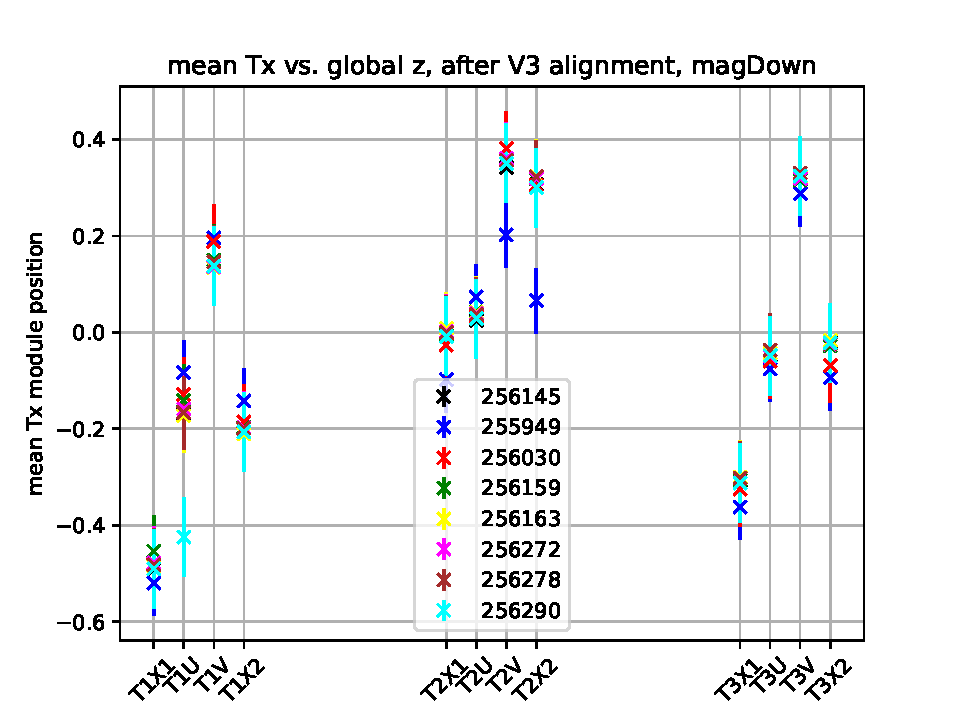
\includegraphics[width=0.9\textwidth]{plots/all_runs_global_z_vs_Tx.pdf}
      \end{figure}
    \end{column}
  \end{columns}
\end{frame}

\begin{frame}\frametitle{Config and run info}
  \begin{columns}
    \begin{column}[c]{0.48\textwidth}
      Config used:
      \begin{itemize}
        \item $\bullet$\, V10 alignment tag
        \item $\bullet$\, DoF: TxTzRz
        \item $\bullet$\, surveyconstraints: data20221115dd4hep
        \item $\bullet$\, lagrange constraints: ["Tx", "Tz", "Rz",
        \item "BackLayerModules: FT/T3/X2/HL.*. : Tx Tz Rx Rz"]
      \end{itemize}
    \end{column}
    \begin{column}[c]{0.48\textwidth}
      \begin{itemize}
        \item $\bullet$\, runs labeled as Good from EMTF
        \item $\bullet$\, fill 8489: blue + red
        \item $\bullet$\, fill 8491: yellow + green + black
        \item $\bullet$\, fill 8496 magenta + brown + cyan
      \end{itemize}
    \end{column}
  \end{columns}
\end{frame}

\begin{frame}\frametitle{module x translation}
  \begin{itemize}
    \item 10 iterations, converged
    \item left plot: module position in comparison to nominal (maximum of 1mm in Tx is expected)
    \item right plot: module position compared to 256145
  \end{itemize}
  \begin{columns}
    \begin{column}[c]{0.48\textwidth}
      \begin{figure}
        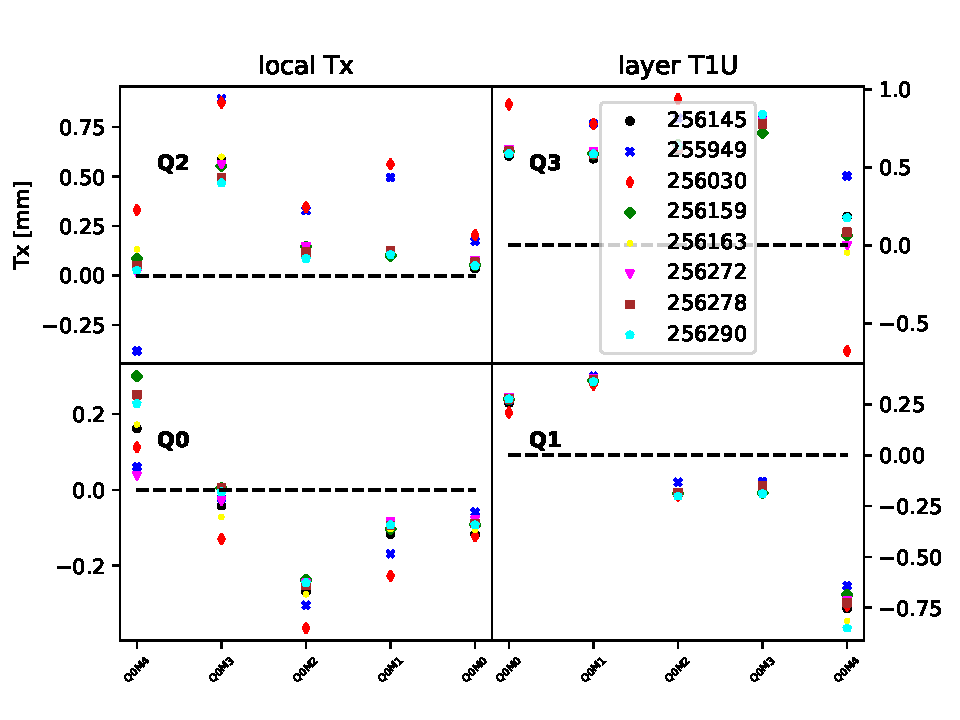
\includegraphics[width=0.9\textwidth]{plots/relative_pos/tx_all_runs_T1U.pdf}
      \end{figure}
    \end{column}
    \begin{column}[c]{0.48\textwidth}
      \begin{figure}
        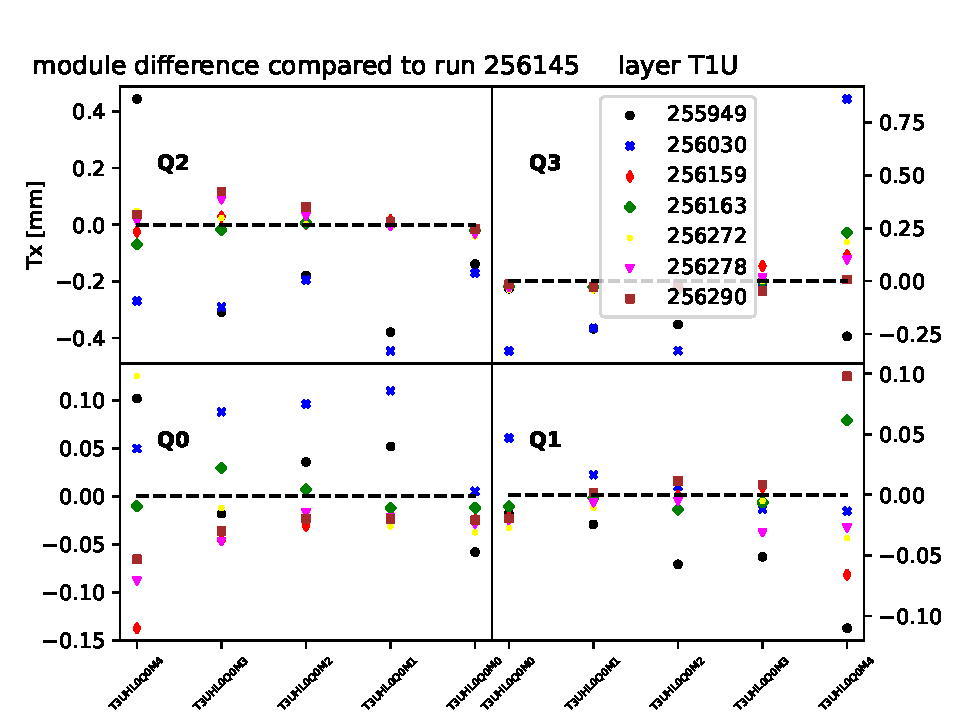
\includegraphics[width=0.9\textwidth]{plots/outfiles_comparison/diff_runs_diff_plots_T1U.pdf}
      \end{figure}
    \end{column}
  \end{columns}
\end{frame}

\begin{frame}\frametitle{nTracks}
  \begin{itemize}
    \item 10 iterations, converged
    \item left plot: module position in comparison to nominal (maximum of 1mm in Tx is expected)
    \item right plot: module position compared to 256145
  \end{itemize}
  \begin{columns}
    \begin{column}[c]{0.48\textwidth}
      \begin{figure}
        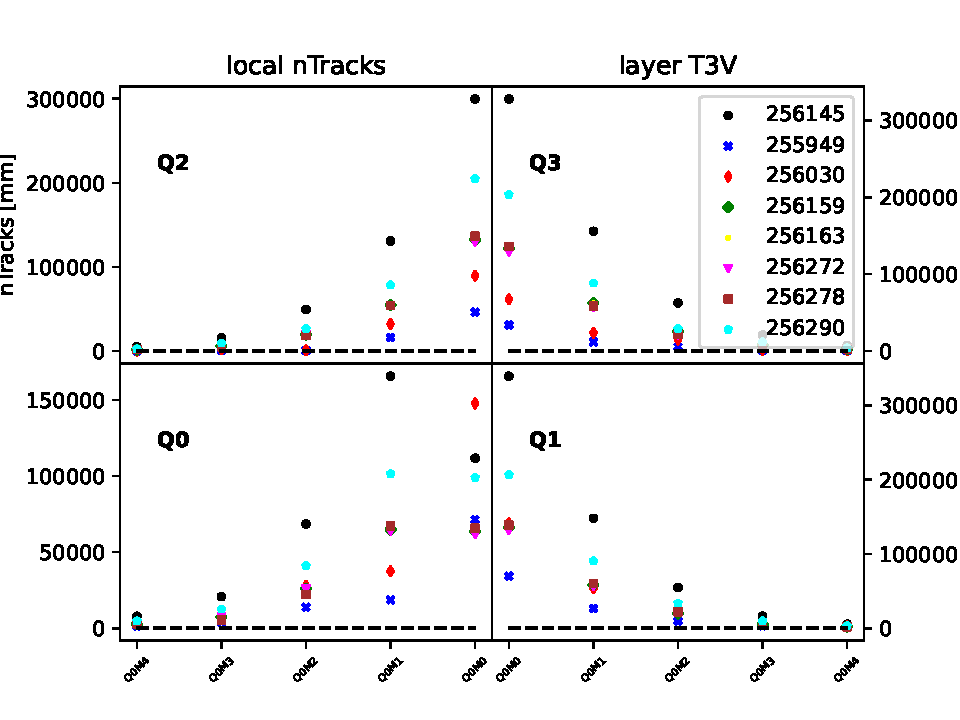
\includegraphics[width=0.9\textwidth]{plots/relative_pos/n_Tracks_T3V.pdf}
      \end{figure}
    \end{column}
    \begin{column}[c]{0.48\textwidth}
      \begin{figure}
        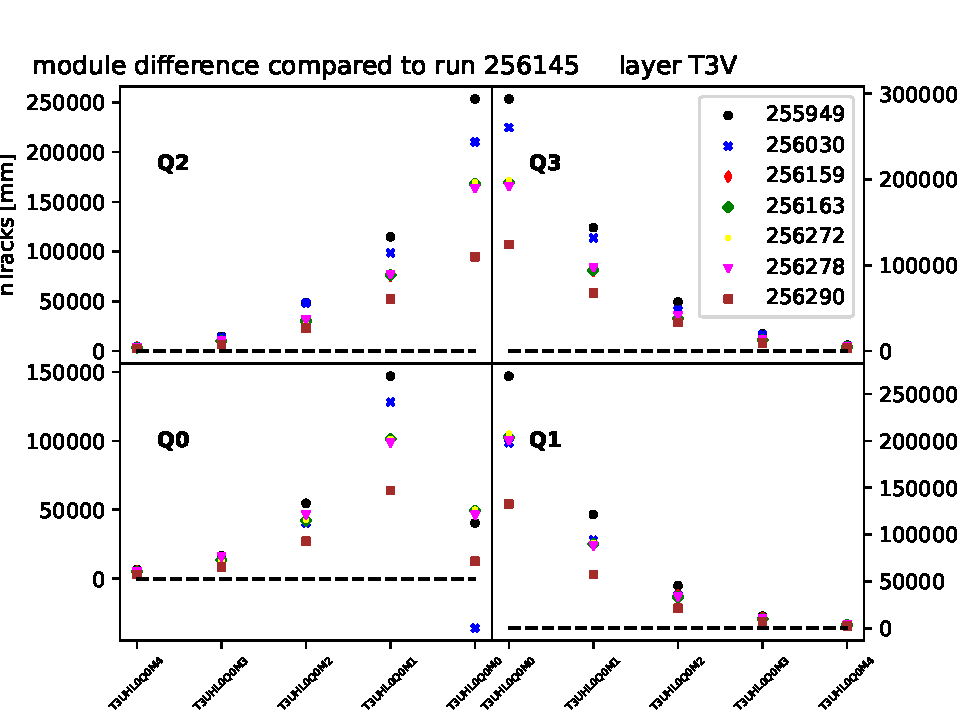
\includegraphics[width=0.9\textwidth]{plots/outfiles_comparison/nTracks_diff_diff_plots_T3V.pdf}
      \end{figure}
    \end{column}
  \end{columns}
\end{frame}

\begin{frame}
  \begin{columns}
    \begin{column}[c]{0.35\textwidth}
      \begin{itemize}
        \item $\bullet$\, 256145, T3V low efficiency in Q0M0
        \item $\bullet$\, module position vs. hit position being off \to not all hits not registered in the module
        \item $\bullet$\, is this just a V10 alignment issue or still visible in v7/v8?
        \item $\bullet$\, Good news: MD and MU runs very comparable
        \item $\bullet$\, Module positions with $\SI{1}{\milli\m}$ in Tx
      \end{itemize}
    \end{column}
    \begin{column}[c]{0.65\textwidth}
      \begin{figure}
        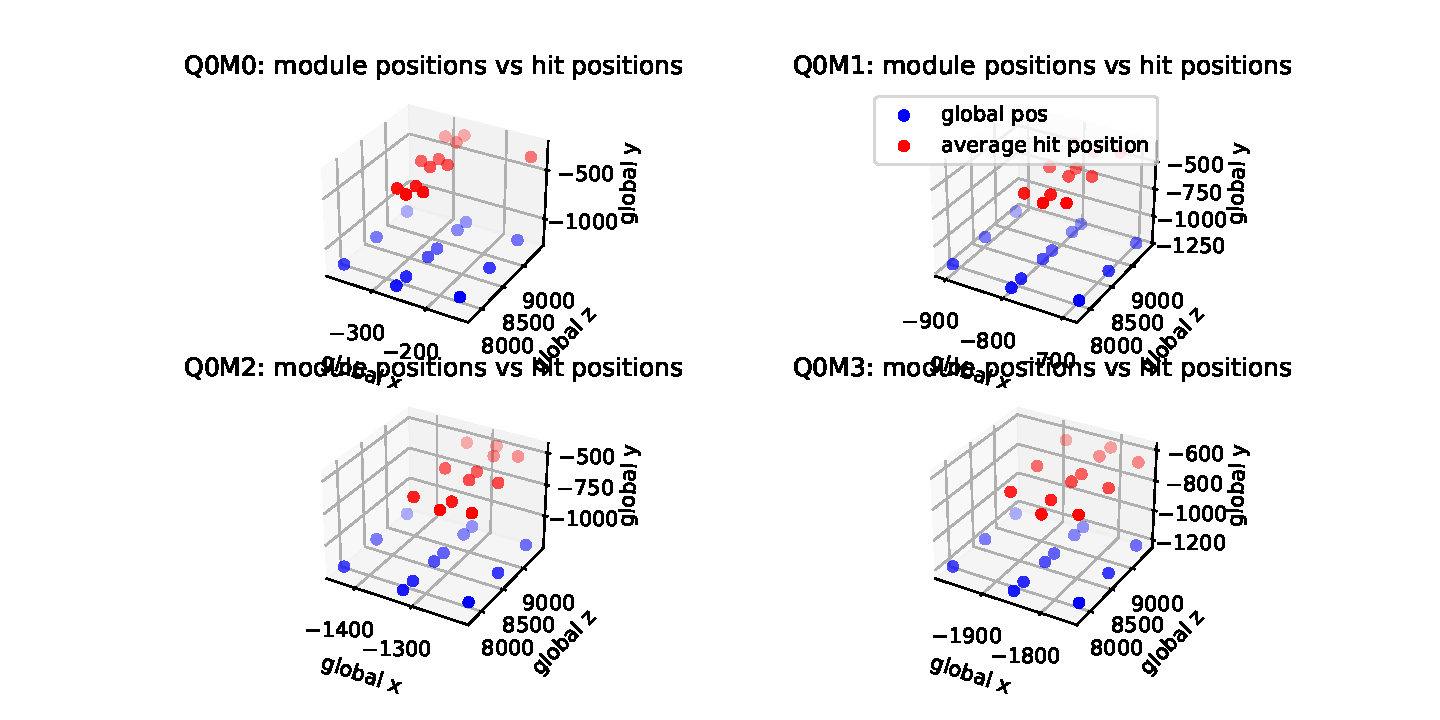
\includegraphics[width=\textwidth]{plots/bad_module_Q0M0.pdf}
      \end{figure}
    \end{column}
  \end{columns}
\end{frame}

\begin{frame}\frametitle{Analysis of joint constraint errors and chi2}
  \begin{columns}
    \begin{column}[c]{0.7\textwidth}
      \begin{itemize}
        \item long modules not in geometry, half modules joined to mimic "banana shape"
        \item combination of 2 Alignables \to how realistic are the errors?
        \item Plan:
        \begin{itemize}
          \item instead of 1 chi2 value calculated from Cov matrix
          \item \to\, calculate chi2 value for each DoF separately
          \item run alignment with different errors and calculate chi2 again
          \item \to\, tune errors to yield more or less chi2/dof = 1
          \item at least make sure none really sticks out
        \end{itemize}
      \end{itemize}
    \end{column}
    \begin{column}[c]{0.3\textwidth}
      % \begin{figure}
      %   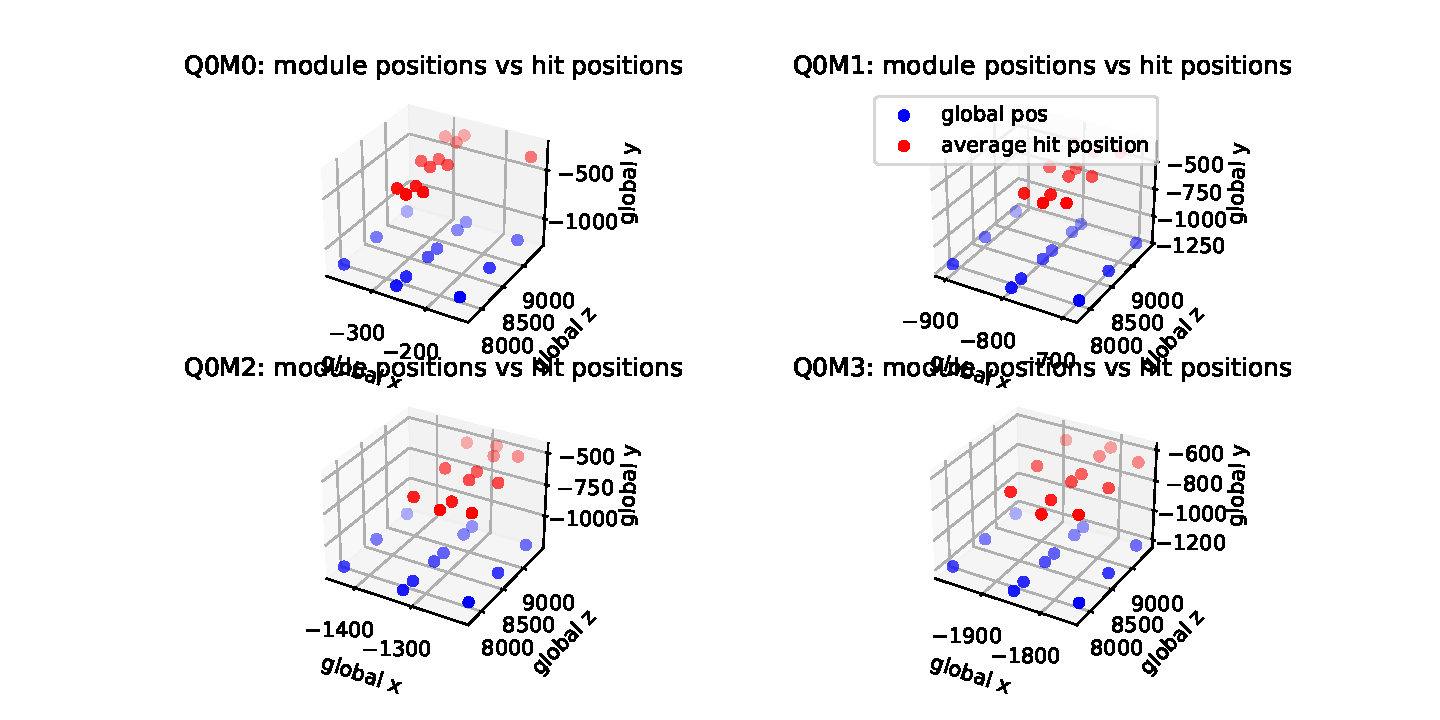
\includegraphics[width=0.9\textwidth]{plots/bad_module_Q0M0.pdf}
      % \end{figure}
    \end{column}
  \end{columns}
\end{frame}

\begin{frame}\frametitle{Analysis of joint constraint errors and chi2}
  \begin{columns}
    \begin{column}[c]{0.5\textwidth}
      \begin{itemize}
        \item $\bullet$\, Covariance matrix: $1 / \text{errors}^2$ diagonal
        \item $\bullet$\, $\chi^2 = (pA - pB)^{T} \cdot \text{Cov} \cdot (pA - pB)$
        \item $\bullet$\, pA, pB: Set of parameters for tophalf- and bottomhalf modules
        \item $\bullet$\, initial errors: (Tx,Ty,Tz,Rx,Ry,Rz)
        \item 0.001 0.001 0.001 0.0002 0.0002 0.0002
      \end{itemize}
    \end{column}
    \begin{column}[c]{0.48\textwidth}
      \begin{figure}
        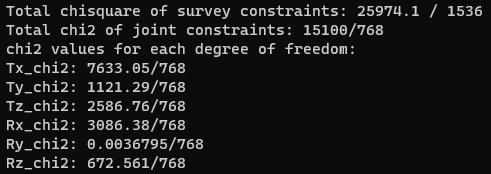
\includegraphics[width=0.9\textwidth]{plots/jointChi2_baseErrors.png}
      \end{figure}
    \end{column}
  \end{columns}
\end{frame}

\begin{frame}\frametitle{Backup}
  \begin{figure}
    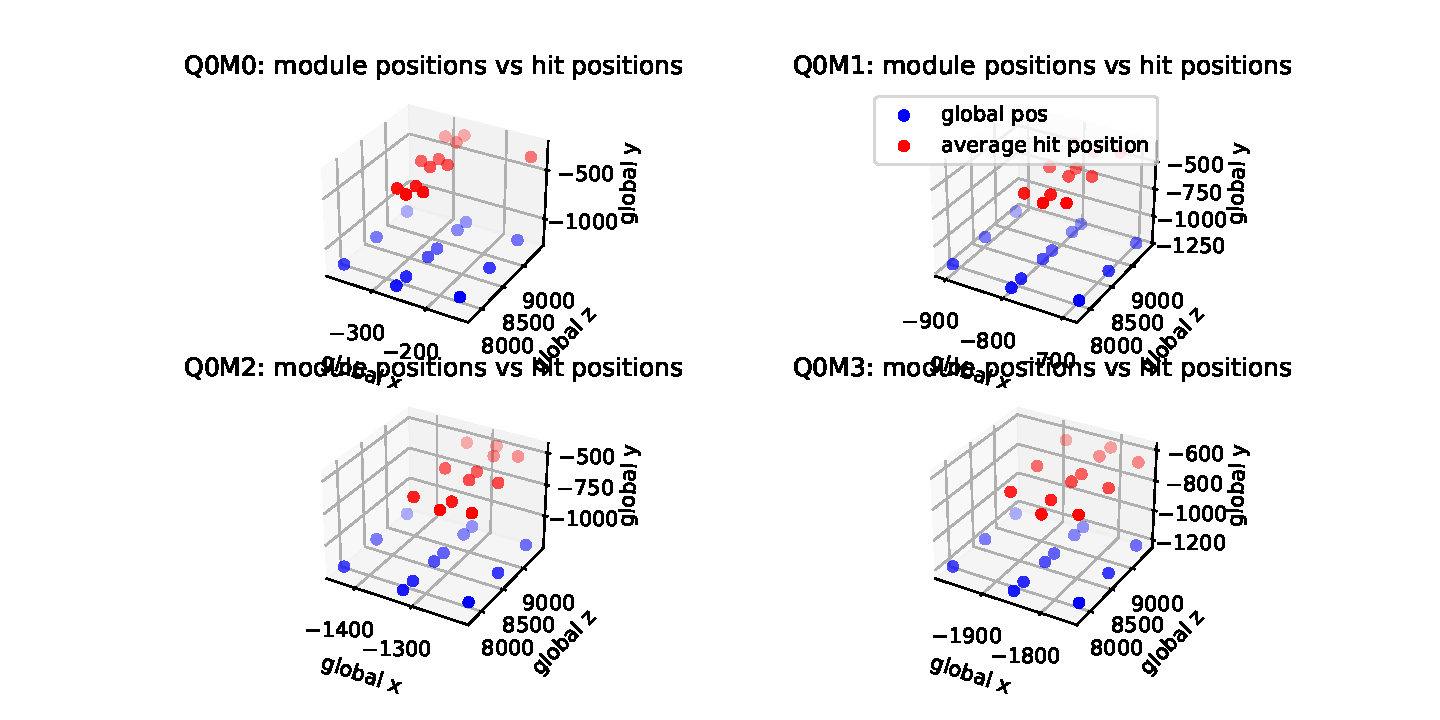
\includegraphics[width=\textwidth]{plots/bad_module_Q0M0.pdf}
  \end{figure}
\end{frame}

\end{document}
